\chapter{Estado del Arte}

Para el desarrollo de este Trabajo de Fin de Grado es necesario utilizar múltiples tecnologías y herramientas. En este capítulo se explicará brevemente el estado actual de los chatbots, las distintas herramientas para desarrollarlos, así como los lenguajes de programación utilizados, qué es el procesamiento natural del lenguaje.


\section{Historia de los chatbots}

Un chatbot es una aplicación de software capaz de mantener una conversación con un usuario dando una serie de respuestas automáticas, establecidas con anterioridad a diferentes entradas que pueda dar el usuario. Existen distintas teorías sobre el origen de los chatbots. 

La primera de ellas, defiende que en la década de 1950, el matemático inglés Alan Turing investigó si una máquina sería capaz de imitar las respuestas de un humano mediante el análisis de una conversación de texto entre un humano y una máquina. 

La segunda, más extendida, sitúa el origen en el año 1966 en el Instituto Tecnológico de Massachusetts (MIT), allí el profesor de informática Joseph Weizenbaum desarrolló en el laboratorio de inteligencia artificial el programa \textit{Eliza}, el concepto es que actuara como si se tratase de un terapeuta. Funcionaba de la siguiente manera: examinaba palabras clave que tenía el enunciado del emisor para poder responder con una serie de oraciones que tenía previamente registradas.

En 1972, surgió el chatbot \textit{Parry}, que simulaba ser una persona con esquizofrenia paranoide. A diferencia de Eliza disponía de una estrategia de comunicación cimentada en premisas y ''respuestas emocionales'' en base a las interacciones con los usuarios. \cite{StreamGenerator}

Como detalle curioso, Eliza y Parry fueron puestos a conversar entre sí mediante la red ARPANET \footnote{ARPANET: red de ordenadores creada por el Departamento de Defensa de los Estados Unidos para conectar varias instituciones académicas y estatales.}  

Posteriormente fue desarrollado \textit{Jabberwacky} por el programador inglés Rollo Carpenter, capaz de mantener una conversación mediante la voz. Aunque fue terminado en 1981 no fue hasta 1997 cuando fue publicado online.

A partir del año 2006 han surgido una gran cantidad de chatbots entre los que cabe destacar:

IBM Watson, nombrado así por el primer director ejecutivo de IBM. En un principio fue desarrollado para responder preguntas y respuestas ideadas por humanos para el concurso Jeopardy. El concurso es el típico de preguntas y respuestas solo que las preguntas son formuladas mediante juegos de palabras y giros lingüisticos. Se presentó al concurso en 2011 por primera vez y fue capaz de ganar a dos especialistas. A partir de ese instante, ha pasado por varias adaptaciones utilizando procesamiento de lenguaje natural y machine learning\footnote{Machine Learning: disciplina dentro de la Inteligencia Artificial que crea sistemas y software capaces de aprender automáticamente} para procesar una gran cantidad de datos. En 2013, IBM anunció que Watson podía ser utilizado para la toma de decisiones en el tratamiento del cáncer de pulmón. 

Tal vez el chatbot más conocido mundialmente sea el asistente virtual desarrollado por Apple, \textit{Siri}. Utiliza consultas dadas mediante comandos de voz para ayudar al usuario de diversas formas, realizar tareas, recordatorios, búsquedas y modificar configuraciones del sistema.

De este mismo estilo tenemos los chatbot \textit{Alexa} creado por Amazon,\textit{Cortana} desarrollado por Microsoft y \textit{Google Now} desarrollado por Google


\section{Frameworks y librerías para el desarrollo de chatbots}

Lo primero qué debemos conocer es la diferencia entre un \textit{Framework} y una librería. Un framework es un tipo de estructura con una serie de archivos y pautas que se utiliza para desarrollar proyectos con una estructura y metodología, es decir, algo así como una plantilla que simplifica la creación de una solución. 
Por otro lado, una librería es uno o varios archivos escritos en algún tipo de lenguaje de programación, que proporcionan varias funcionalidades. Al contrario que un framework, una librería no establece la estructura sobre cómo debe realizarse el desarrollo, sino que da funcionalidades genéricas que han sido programadas con anterioridad y evitan que haya que escribir código de más, aumentando la calidad del código y reduciendo el tiempo de desarrollo.

\section{Frameworks}

\subsection{DialogFlow}
Framework de desarrollo de chatbots creado en 2010 y mantenido por Google\cite{Dialogflow}. Es capaz de comprender el lenguaje natural y nos brinda herramientas para la fabricación de diálogos y la recreación de conversaciones. Destaca por la gran cantidad de interfaces de conversación en los que se puede desplegar (Google home, google assistant, wereables, teléfonos, coches). Tiene soporte para más de 14 idiomas y es capaz de resolver abreviaturas y funcionar con faltas de ortografía. 
Posee una interfaz muy intuitiva y permite crear chatbots en una cantidad pequeña de tiempo. 
\begin{figure}[ht]
    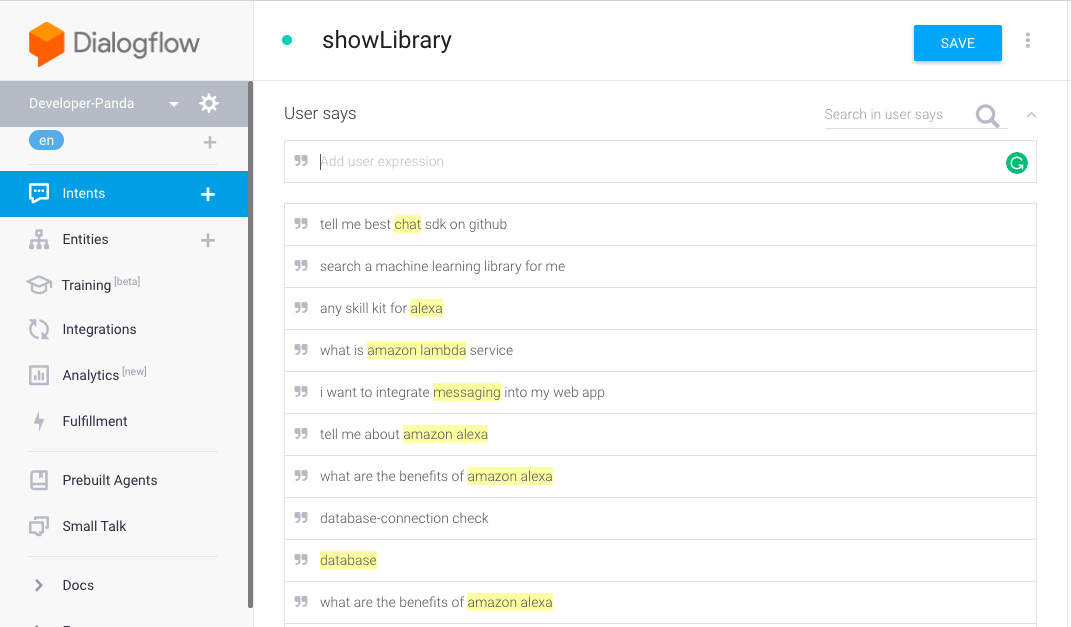
\includegraphics[width=\textwidth]{{include/figuras/DialogFlow.png}}
    \caption{Interfaz de dialogflow}
    \label{fig:dialogflow_gui}
\end{figure}


\subsection{Microsoft Bot Framework}
Desarrollado por Microsoft, crea chatbots rapidamente a través de la herramienta Microsoft Bot Builder y los conecta con Azure Bot Service, lo que nos permite una rápida creación del bot ya que nos proporciona diversas plantillas para seleccionar cuando se está creando el bot y nos brinda todas las mejoras de la nube creada por Microsoft. Puede editarse con directamente desde la página web usando el editor de Azure o algún IDE de desarrollo como Visual Studio o Visual Studio Code \cite{MicrosoftBotBuilder}. Posee su propio sistema de procesamiento natural del lenguaje llamado LUIS (\textit{Language Understanding Intelligent Service}).   

\subsection{IBM Watson}
Creado por IBM, es capaz de comprender y responder a las preguntas de los usuarios mediante lenguaje natural \cite{MicrosoftBotBuilder}. Watson está compuesto actualmente por un clúster de al menos 750 servidores \textit{IBM Power 750}, con unos 16 TB de memoria RAM, lo que proporciona una potencia de cálculo bruto de unos \textbf{80 petaflops}, convirtiéndolo así en uno de los supercomputadores más potentes del mundo. 

\subsection{Amazon Lex}
Creado y gestionado por Amazon, permite establecer comuncicaciones con todos sus productos Eco y con su asistente virtual Alexa. Es una de las mejores herramientas en cuanto a conversión de voz a texto. Con esta herramienta se pueden crear bots con un lenguaje natural sofisticado. A diferencia de los anteriores, tiene una interfaz más intuitiva para principiantes aunque por el contrario, dispone de menos herramientas, aunque posee todas las necesarias en un chatbot.

\subsection{Rasa}
Por último cabe destacar Rasa, una framework \textit{Open Source} de machine learning que nos permite crear conexiones entre las máquinas y el usuario. Posee herramientas para entender al usuario mediante el componente Rasa NLU (Natural Langugage Understanding), generar el diálogo con Rasa NLG (Natural Language Generation) y un motor (Rasa Core) capaz de definir cuál será la siguiente acción a tomar en función del mensaje transmitido por el usuario.   

\vspace{1cm}
\section{Librerías}
Vamos a analizar las librerías existentes para el lenguaje de programación Python, debido a que se trata de un lenguaje simple, elegante ordenado y portable.

\subsection{Chatterbot}
Se trata de una librería de machine learning basada en las conversaciones y diálogos tradicionales. Lo más destacable de esta librería es que está diseñada de tal manera que permite crear chatbots que soporten varios idiomas. 

Es también compatible con librerías para aportar más funcionalidades como puede ser la conversión de texto a voz y así poder interactuar con el usuario sin necesidad de escribir.

\subsection{Natural Language ToolKit} NTLK por sus siglas en inglés, se trata de una plataforma para crear chatbots con lenguaje humano. Dispone de funcionalidades muy interesantes desde el punto de vista del reconocimiento del lenguage como la tokenización , derivación, etiquetado, análisis y razonamiento semántico.

\subsection{ChatbotAI} Nos permite crear un chatbot con muy pocas líneas de código. Genera un controlador del chat y bots con inteligencia artificial que permiten una integración muy sencilla con API Rest. Esta inteligencia artificial nos genera múltiples características como aprender, memorizar, manejar conversaciones según el tema \cite{chatbotAI}. 

\subsection{Tensorflow} Es uan plataforma de código abierto gestionada por Google. Se trata de una biblioteca de aprendizaje automático con la que es posible construir y entrenar redes neuronales para detectar patrones y correlaciones en el aprendizaje y razonamiento de los humanos. 